\documentclass[]{article}
\usepackage{lmodern}
\usepackage{amssymb,amsmath}
\usepackage{ifxetex,ifluatex}
\usepackage{fixltx2e} % provides \textsubscript
\ifnum 0\ifxetex 1\fi\ifluatex 1\fi=0 % if pdftex
  \usepackage[T1]{fontenc}
  \usepackage[utf8]{inputenc}
\else % if luatex or xelatex
  \ifxetex
    \usepackage{mathspec}
  \else
    \usepackage{fontspec}
  \fi
  \defaultfontfeatures{Ligatures=TeX,Scale=MatchLowercase}
\fi
% use upquote if available, for straight quotes in verbatim environments
\IfFileExists{upquote.sty}{\usepackage{upquote}}{}
% use microtype if available
\IfFileExists{microtype.sty}{%
\usepackage{microtype}
\UseMicrotypeSet[protrusion]{basicmath} % disable protrusion for tt fonts
}{}
\usepackage[margin=1in]{geometry}
\usepackage{hyperref}
\hypersetup{unicode=true,
            pdftitle={Graphics},
            pdfauthor={Kayla Frisoli, Shannon Gallagher, and Amanda Luby},
            pdfborder={0 0 0},
            breaklinks=true}
\urlstyle{same}  % don't use monospace font for urls
\usepackage{longtable,booktabs}
\usepackage{graphicx,grffile}
\makeatletter
\def\maxwidth{\ifdim\Gin@nat@width>\linewidth\linewidth\else\Gin@nat@width\fi}
\def\maxheight{\ifdim\Gin@nat@height>\textheight\textheight\else\Gin@nat@height\fi}
\makeatother
% Scale images if necessary, so that they will not overflow the page
% margins by default, and it is still possible to overwrite the defaults
% using explicit options in \includegraphics[width, height, ...]{}
\setkeys{Gin}{width=\maxwidth,height=\maxheight,keepaspectratio}
\IfFileExists{parskip.sty}{%
\usepackage{parskip}
}{% else
\setlength{\parindent}{0pt}
\setlength{\parskip}{6pt plus 2pt minus 1pt}
}
\setlength{\emergencystretch}{3em}  % prevent overfull lines
\providecommand{\tightlist}{%
  \setlength{\itemsep}{0pt}\setlength{\parskip}{0pt}}
\setcounter{secnumdepth}{5}
% Redefines (sub)paragraphs to behave more like sections
\ifx\paragraph\undefined\else
\let\oldparagraph\paragraph
\renewcommand{\paragraph}[1]{\oldparagraph{#1}\mbox{}}
\fi
\ifx\subparagraph\undefined\else
\let\oldsubparagraph\subparagraph
\renewcommand{\subparagraph}[1]{\oldsubparagraph{#1}\mbox{}}
\fi

%%% Use protect on footnotes to avoid problems with footnotes in titles
\let\rmarkdownfootnote\footnote%
\def\footnote{\protect\rmarkdownfootnote}

%%% Change title format to be more compact
\usepackage{titling}

% Create subtitle command for use in maketitle
\newcommand{\subtitle}[1]{
  \posttitle{
    \begin{center}\large#1\end{center}
    }
}

\setlength{\droptitle}{-2em}

  \title{Graphics}
    \pretitle{\vspace{\droptitle}\centering\huge}
  \posttitle{\par}
    \author{Kayla Frisoli, Shannon Gallagher, and Amanda Luby}
    \preauthor{\centering\large\emph}
  \postauthor{\par}
    \date{}
    \predate{}\postdate{}
  
\usepackage{booktabs}
\usepackage{longtable}
\usepackage{array}
\usepackage{multirow}
\usepackage[table]{xcolor}
\usepackage{wrapfig}
\usepackage{float}
\usepackage{colortbl}
\usepackage{pdflscape}
\usepackage{tabu}
\usepackage{threeparttable}
\usepackage{threeparttablex}
\usepackage[normalem]{ulem}
\usepackage{makecell}

\begin{document}
\maketitle

\subsection{Is being a winner from Spain independent of
tournament?}\label{is-being-a-winner-from-spain-independent-of-tournament}

\begin{center}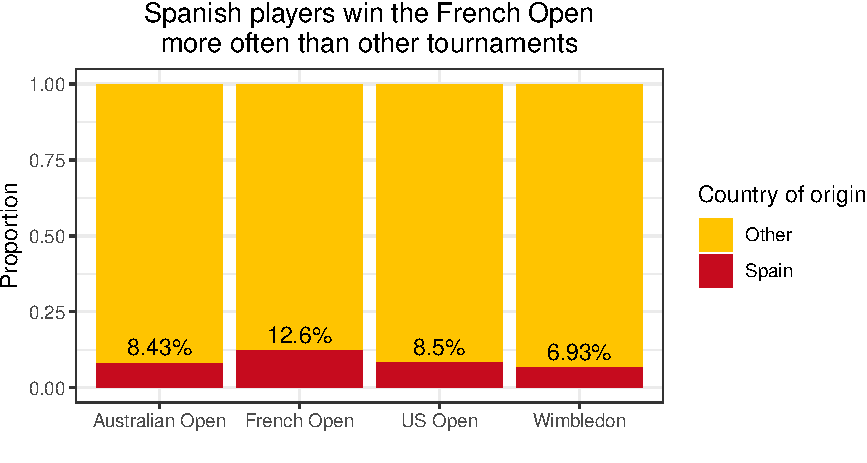
\includegraphics{graphics_files/figure-latex/unnamed-chunk-1-1} \end{center}

\begin{table}[!htb]
    \begin{minipage}{.5\linewidth}
      \caption{Actual table}
      \centering 
\begin{tabular}{lrr}
\toprule
  & Other & Spain\\
\midrule
Australian Open & 1163 & 107\\
French Open & 1110 & 160\\
US Open & 1162 & 108\\
Wimbledon & 1182 & 88\\
\bottomrule
\end{tabular} \end{minipage}%
    \begin{minipage}{.5\linewidth}
      \centering
        \caption{Expected table} 
\begin{tabular}{lrr}
\toprule
  & Other & Spain\\
\midrule
Australian Open & 1154.25 & 115.75\\
French Open & 1154.25 & 115.75\\
US Open & 1154.25 & 115.75\\
Wimbledon & 1154.25 & 115.75\\
\bottomrule
\end{tabular} \end{minipage} 
\end{table}

\begin{longtable}[]{@{}ccc@{}}
\caption{Pearson's Chi-squared test:
\texttt{spain\_vs\_tourn}}\tabularnewline
\toprule
\begin{minipage}[b]{0.22\columnwidth}\centering\strut
Test statistic\strut
\end{minipage} & \begin{minipage}[b]{0.06\columnwidth}\centering\strut
df\strut
\end{minipage} & \begin{minipage}[b]{0.22\columnwidth}\centering\strut
P value\strut
\end{minipage}\tabularnewline
\midrule
\endfirsthead
\toprule
\begin{minipage}[b]{0.22\columnwidth}\centering\strut
Test statistic\strut
\end{minipage} & \begin{minipage}[b]{0.06\columnwidth}\centering\strut
df\strut
\end{minipage} & \begin{minipage}[b]{0.22\columnwidth}\centering\strut
P value\strut
\end{minipage}\tabularnewline
\midrule
\endhead
\begin{minipage}[t]{0.22\columnwidth}\centering\strut
27.23\strut
\end{minipage} & \begin{minipage}[t]{0.06\columnwidth}\centering\strut
3\strut
\end{minipage} & \begin{minipage}[t]{0.22\columnwidth}\centering\strut
5.265e-06 * * *\strut
\end{minipage}\tabularnewline
\bottomrule
\end{longtable}


\end{document}
